\documentclass[8pt]{beamer}

\usetheme{Copenhagen}
\usecolortheme{beaver}
\usepackage[small,center]{caption}
\usepackage{times}
\usefonttheme{structurebold}
\usepackage[english]{babel}
\usepackage{pgf,pgfarrows,pgfnodes,pgfautomata,pgfheaps}
\usepackage{amsmath,amssymb}
\usepackage{amsxtra}

\usepackage{caption}

\newcommand{\leftd}[1]{{\color{red} \bar{#1}}}
\newcommand{\interface}[2]{{\color{blue}{#1}_I(#2)}}
\newcommand{\leftdd}[2]{{\color{red} \bar{#1}(\bar{#2})}}
\newcommand{\half}{\dfrac{1}{2}}
\newcommand{\divergence}{\mathrm{div}}

\newcommand*{\vcenterimage}[1]{\vcenter{\hbox{\includegraphics[width=2in]{#1}}}}
\newcommand*{\vcenterarrow}{\vcenter{\hbox{$\Longrightarrow$}}}


\definecolor{RPIred}{rgb}{ 0.87,0.12, 0.20}
\definecolor{ballblue}{rgb}{0.13, 0.67, 0.8}
\definecolor{lightgray}{rgb}{0.83, 0.83, 0.83}
\setbeamercolor{block title}{bg=lightgray,fg=RPIred}
\setbeamercolor{block body}{bg=white,fg=black}
\setbeamercovered{dynamic}
\setbeamercolor*{item}{fg=RPIred}

\captionsetup[subfigure]{labelformat=empty}
\captionsetup[figure]{labelformat=empty}
\setbeamertemplate{navigation symbols}{}
\setbeamertemplate{footline}[frame number]
\begin{document}

\frame{
\title{\Large Partitioned Fluid Structure Interactions for Stokes Flow Problems}

\author{{\Large David Wells \\\vspace{0.1in} Rensselaer Polytechnic Institute}\\
\vspace{0.2in} {In collaboration with:\\{}J. W. Banks, F. Li}}

\date{July 6, 2016\\{}PDESOFT                                                 \\
Warwick University}

\begin{figure}[h]
\centering
\includegraphics[width=1.5in]{RPI_letterhead.pdf}
 \end{figure}%

\vspace{-0.2in}
\titlepage
}

\begin{frame}
    \frametitle{Outline}
    \begin{itemize}
    \item[$\blacksquare$]  Definitions and Goals                              \\
    \item[$\blacksquare$]  Governing Equations                                \\
    \item[$\blacksquare$]  Added Mass Partition (AMP) Scheme                  \\
    \item[$\blacksquare$]  Finite Element Scheme                              \\
    \item[$\blacksquare$]  Numerical Results                                  \\
    \item[$\blacksquare$]  Summary                                            \\
    \end{itemize}
\end{frame}

\begin{frame}
    \frametitle{Renssel-where?}

    \begin{figure}
        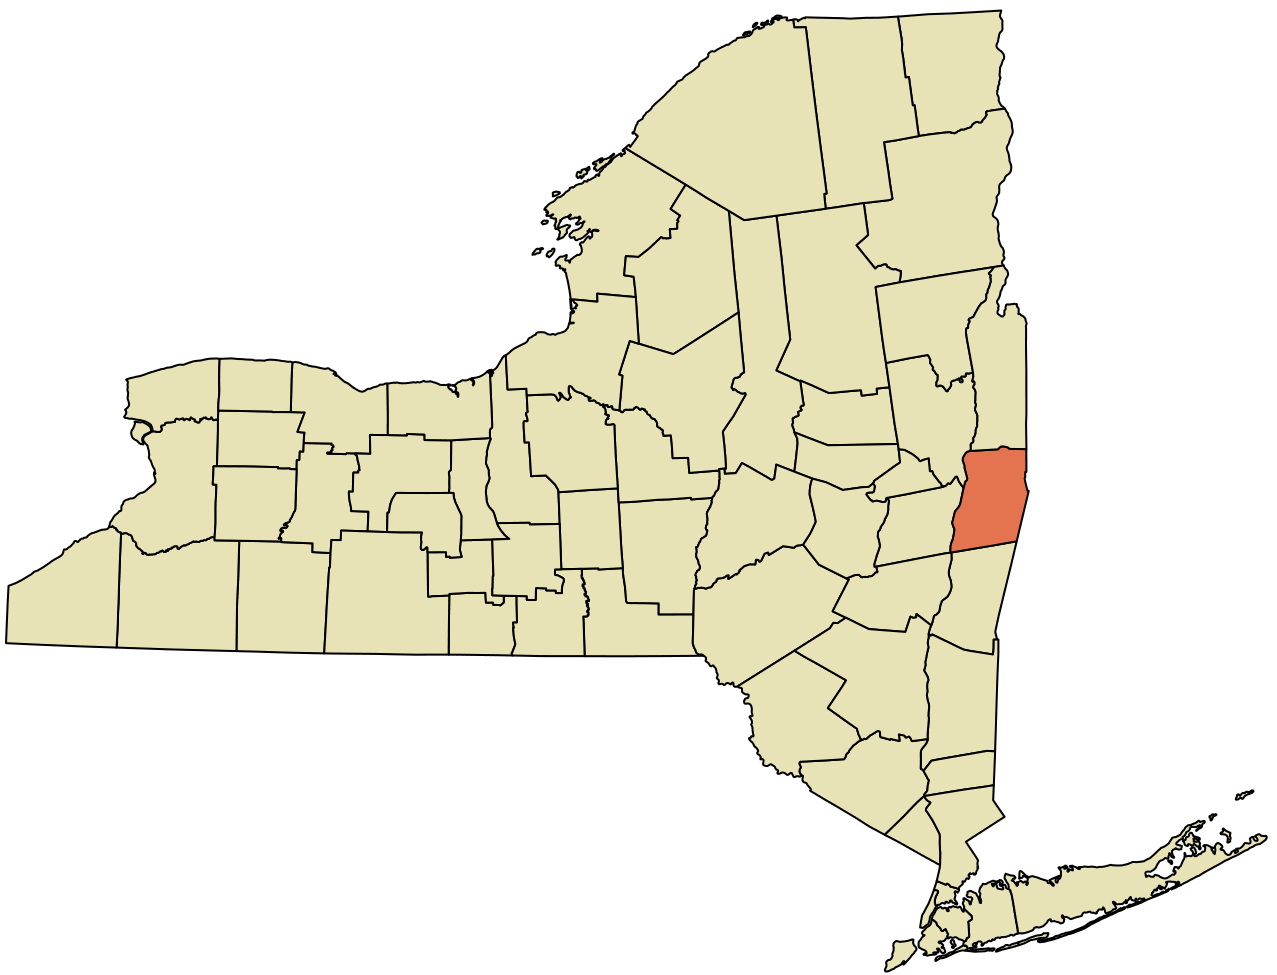
\includegraphics[width=3in]{rensselaer.png}

        \caption{Rensselaer County, the location of RPI, is in red.}
    \end{figure}
\end{frame}

\begin{frame}
    \frametitle{Partitioned Methods}
    \emph{Partitioned Methods} couple a fluid and structure solver along a
    specified interface. They are an alternative option to \emph{monolithic
    solvers}, which advance both the structure and the fluid in one joint
    system.
\end{frame}

\begin{frame}
    \frametitle{Goals \& Dreams}
    \begin{itemize}
        \item Reuse existing fluid and structure codes (without complete
              rewrites)
        \item Reasonable time step constraints
        \item No need for subiterations for stability
        \item Arbitrarily high order accuracy
    \end{itemize}
\end{frame}

\begin{frame}
    \frametitle{Governing Equations}
    incompressible fluid:
    \begin{align}
        \rho \vec{v}_t &= \divergence \sigma + \vec{f}                        \\
        \sigma &= -p I + 2 \nu \varepsilon(v)                                 \\
        \varepsilon(\vec{v})_{ij} &= \dfrac{1}{2}
        \left(
        \dfrac{\partial v_i}{\partial x_j} +
        \dfrac{\partial v_j}{\partial x_i}
        \right)                                                               \\
        \divergence \vec{v} &= 0
    \end{align}

    thin shell, i.e., a beam:
    \begin{align}
        \leftd{u}_t              &= \leftd{v}                                 \\
        \leftd{\rho} \leftd{v}_t &= \leftdd{L}{u} + \leftd{b} + \leftd{f}
    \end{align}

    \pause
    coupling:
    \begin{align}
        v &= \leftd{v} \text{ (at the interface)}                             \\
        \leftd{b} &= -\sigma n.
    \end{align}
    \pause

    Applying the physical boundary condition as the numerical one is usually
    called the \emph{traditional scheme}.
\end{frame}

\begin{frame}
    \frametitle{Governing Equations}
    The physical boundary conditions are a source of instability when the beam
    is very light.

    \begin{figure}
        \centering
        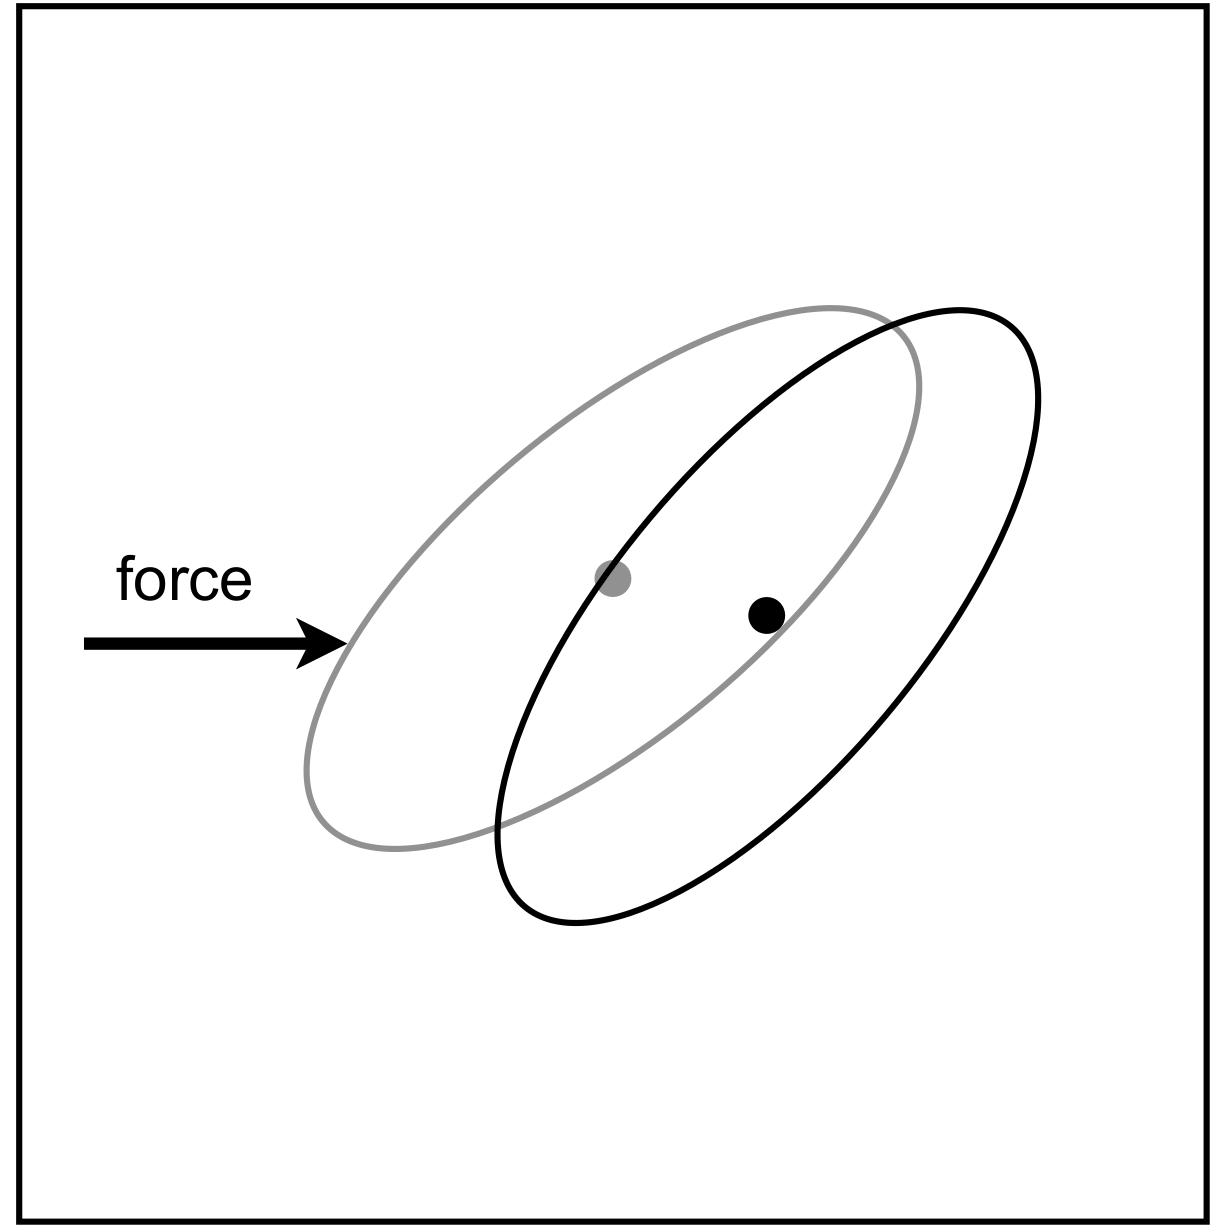
\includegraphics[width=2.25in]{left.png}

        \caption{A solid moving in a vacuum displaces no mass.}
    \end{figure}
\end{frame}

\begin{frame}
    \frametitle{Governing Equations}
    The physical boundary conditions are a source of instability when the beam
    is very light.

    \begin{figure}
        \centering
        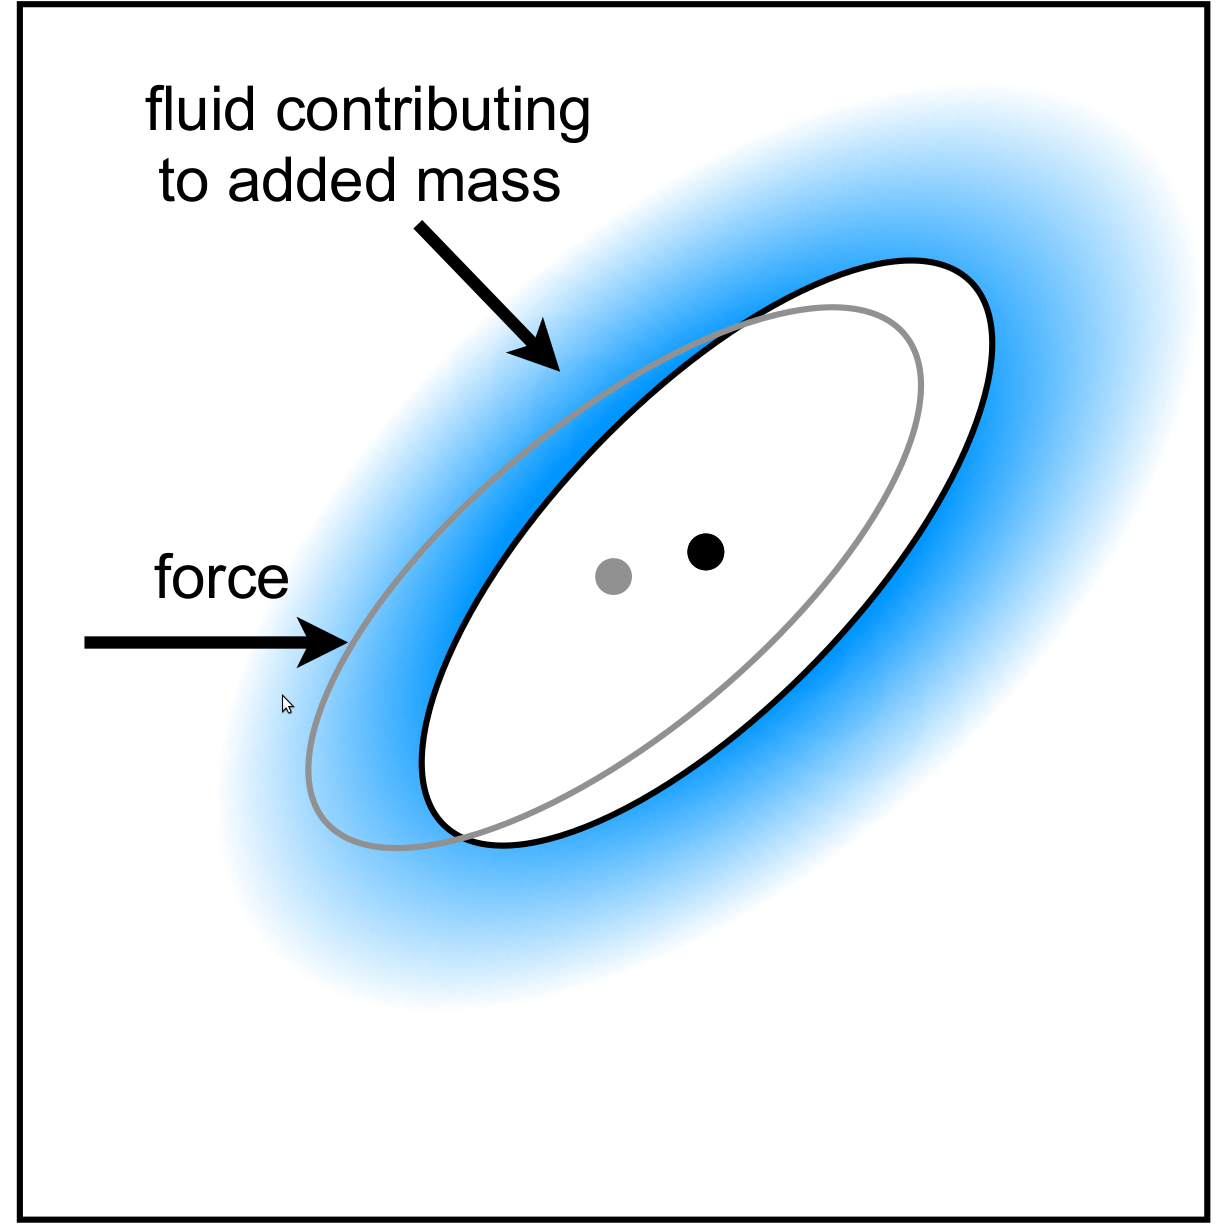
\includegraphics[width=2.25in]{right.png}

        \caption{A solid moving in a fluid must displace and entrain part of the
        fluid.}
    \end{figure}
\end{frame}

\begin{frame}
    \frametitle{Previous Work}
    Most of the work has been done for finite differences with overlapping
    grids.

    \begin{figure}
        \centering

        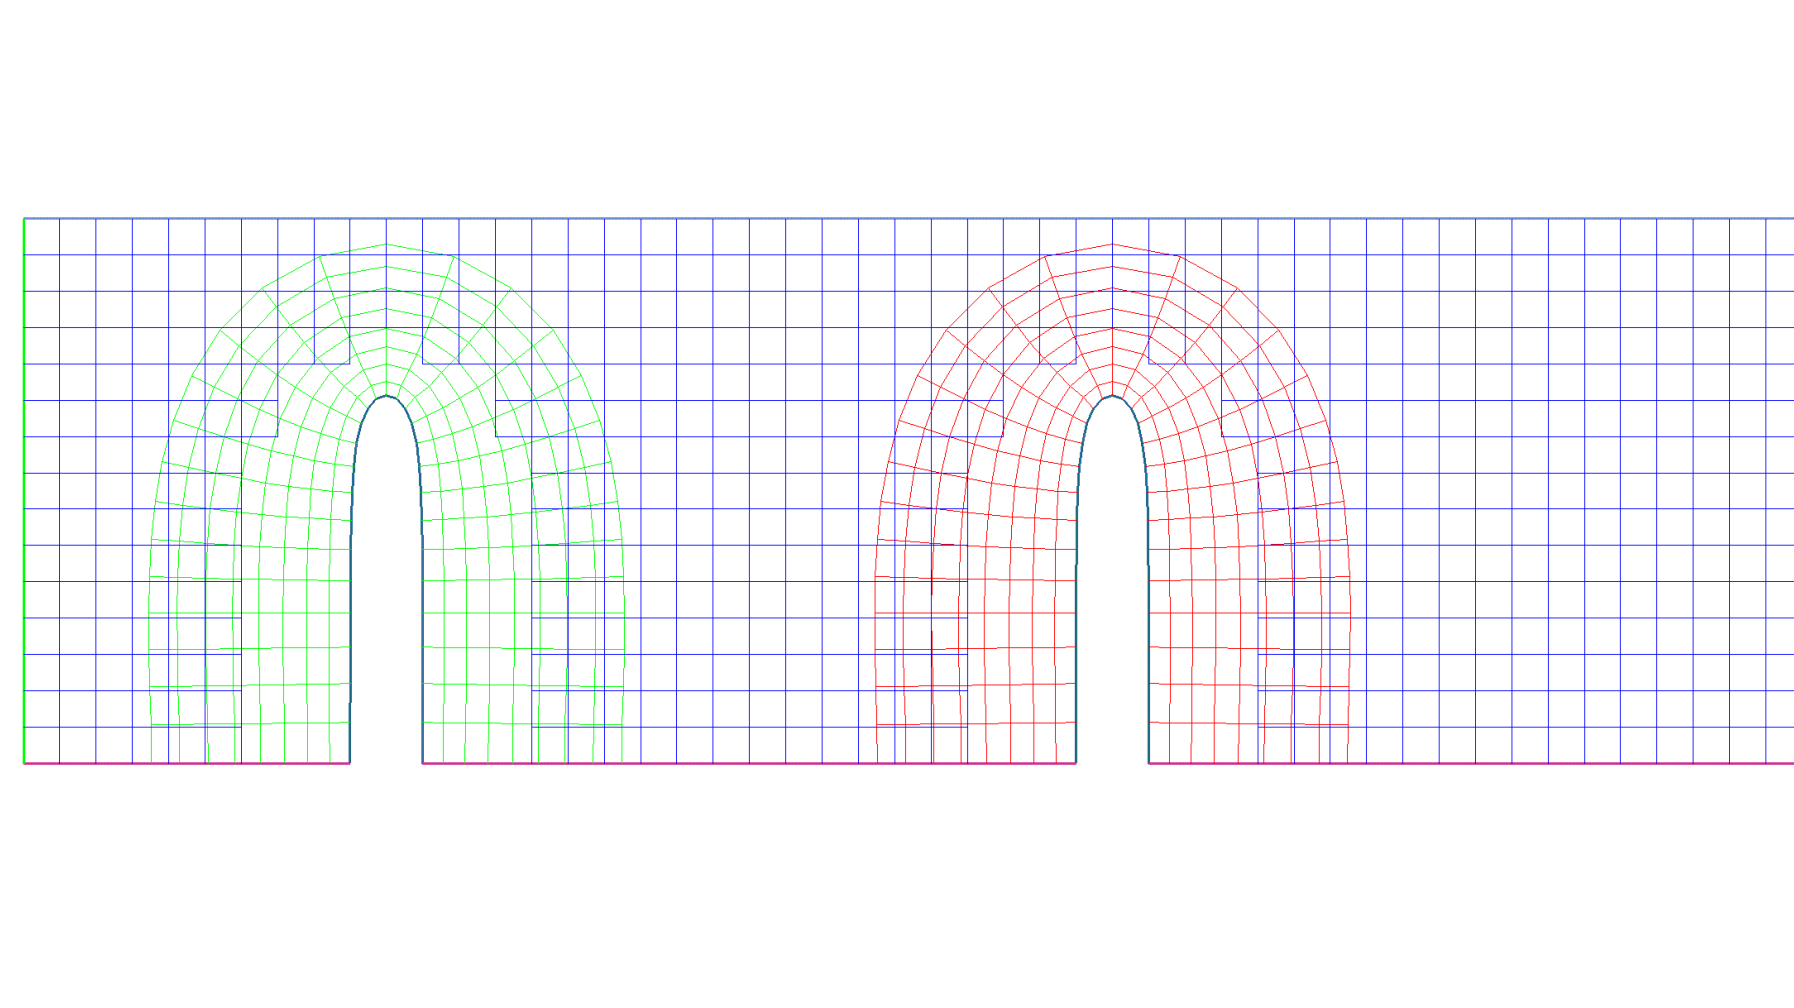
\includegraphics[width=3in]{longfei.png}

        \caption{Coarse grid of a channel with two protruding beams. Curvilinear
        grids describe the domain near the structures while the background
        Cartesian grid describes most of the domain.}
    \end{figure}
\end{frame}

\begin{frame}
    \frametitle{Traditional Coupling}
    \emph{Traditional Coupling} refers to using the physical boundary conditions
    for the numerical solver.

    With some simplifying assumptions on the fluid (periodic in the non-shell
    direction, zero viscosity) we can explicitly compute the mode-dependent
    added mass:
    \begin{equation}
        M_{a,k} = \dfrac{\rho L}{2 \pi k} \coth(2 \pi k H / L)
    \end{equation}
    where \(H\) is the height of the fluid domain and \(L\) is the length (the
    beam is at the \(y = H\) boundary).

    \pause
    By a result from von Neumann polynomials the traditional scheme is only
    stable if
    \begin{align}
        M_a &< \leftd{\rho} \leftd{h}                                         \\
        \Delta t^2 &< 4 \dfrac{\leftd{\rho} \leftd{h}}{\leftd{\mathcal{L}}}
        \left[1 - \dfrac{M_a}{\leftd{\rho} \leftd{h}}\right]
    \end{align}
    where \(\leftd{\rho}\), \(\leftd{h}\), and \(\leftd{\mathcal{L}}\) are
    physical beam constants. The time stepping algorithms are backward Euler for
    the fluid and leapfrog for the beam.
\end{frame}

\begin{frame}
    \frametitle{AMP Coupling}
    Some beams are sufficiently light that (for the simplified model) that there
    is no stable time step choice with the traditional scheme.
    \pause
    \begin{align}
        \leftd{\rho} \leftd{h} \leftd{v_t}
        &= \leftdd{\mathcal{L}}{u} + \leftd{f} - \sigma n                     \\
        \leftd{\rho} \leftd{h} v_t
        &= \leftdd{\mathcal{L}}{u} + \leftd{f} - \sigma n                     \\
        \dfrac{\leftd{\rho} \leftd{h}}{\rho} \divergence(\sigma)
        + \dfrac{\leftd{\rho} \leftd{h}}{\rho} f
        &= \leftdd{\mathcal{L}}{u} + \leftd{f} - \sigma n
    \end{align}
    or, more simply
    \begin{equation}
        \sigma n + \dfrac{\leftd{\rho} \leftd{h}}{\rho} \divergence(\sigma)
        = \leftdd{\mathcal{L}}{u}
        + \leftd{f}
        - \dfrac{\leftd{\rho} \leftd{h}}{\rho} f.
    \end{equation}
\end{frame}

\begin{frame}
    \frametitle{AMP Coupling}
    For the same model problem we now get a time step constraint (again by von
    Neumann polynomials) of
    \begin{equation}
        \Delta t < 2
        \sqrt{\dfrac{\leftd{\rho} \leftd{h} (1 + M_a)}{\leftd{\mathcal{L}}}}
    \end{equation}
\end{frame}

\begin{frame}
    \frametitle{What does this mean for finite elements?}
    An open area: compatibility boundary conditions (using the PDE at the
    boundary) is much more common for finite differences than finite elements.

    \pause
    \vspace{0.5in}
    After integrating by parts over the domain \(\Omega\):
    \begin{align}
        \rho (\varphi, \vec{v}_t) &= -(\nabla \varphi, \sigma)
        + (\varphi, \sigma n)_{\partial \Omega}
        + (\varphi, f)                                                        \\
        (q, \divergence(v)) &= 0
    \end{align}

    so replace the normal part of the traction with the PDE:
    \begin{equation}
        (\varphi, \sigma n)_{\partial \Omega} = \left(\varphi,
        - \dfrac{\leftd{\rho} \leftd{h}}{\rho} \divergence(\sigma)
        + \leftdd{\mathcal{L}}{u}
        + \leftd{f}
        - \dfrac{\leftd{\rho} \leftd{h}}{\rho} f\right)_{\partial \Omega}
    \end{equation}
\end{frame}

\begin{frame}
    \frametitle{What does this mean for finite elements?}
    Simplifications:
    \begin{itemize}
        \item Only enforce this AMP condition in the normal direction (e.g., use
              Dirichlet conditions tangentially)
        \item Assume that the beam solution is already known, i.e., enforce
              \begin{equation}
                  \sigma n + \divergence(\sigma) = g
              \end{equation}
              on the boundary.
    \end{itemize}
\end{frame}

\begin{frame}
    \frametitle{\(2D\) Numerical Experiments}
    \begin{itemize}
        \item \(Q^3-Q^2\) elements
        \item \(\Delta x = 1/50\)
        \item Unit square: the AMP condition is enforced along the top
        \item Velocity-divergence form
        \item Trapezoid rule time step
        \item \(\Delta t = \Delta x^2\)
    \end{itemize}
    with exact solution
    \begin{align}
        \psi(t, x, y) &= t y^2                                                \\
        p(t, x, y)    &= t x y
    \end{align}
\end{frame}

\begin{frame}
    \frametitle{\(2D\) Numerical Experiments}
    \begin{figure}
        \centering
        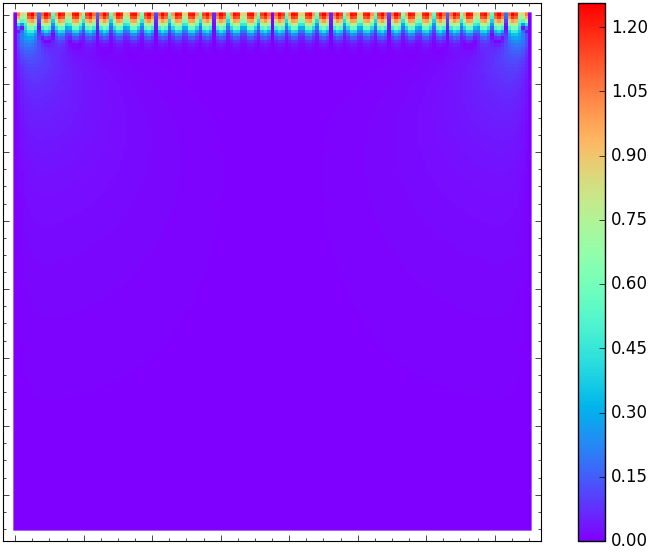
\includegraphics[width=3in]{v1-10.png}

        \caption{Magnitude in the error after ten time steps.}
    \end{figure}
\end{frame}

\begin{frame}
    \frametitle{\(2D\) Numerical Experiments}
    \begin{figure}
        \centering
        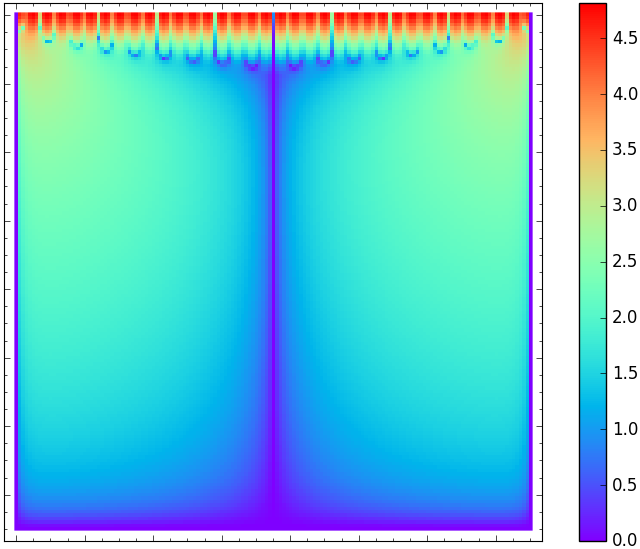
\includegraphics[width=3in]{v1-12.png}

        \caption{Magnitude in the error after twelve time steps.}
    \end{figure}
\end{frame}

\begin{frame}
    \frametitle{Dealing with the instability}
    Implementing the AMP boundary, even with integration by parts, requires
    derivative information at the boundary which may not exist: a workaround is
    to use elements with some derivative information.

    \begin{figure}
        \begin{equation*}
            \vcenterimage{lagrange-quadratics.png}
            \vcenterarrow
            \vcenterimage{hermite-quadratics.png}
        \end{equation*}
    \end{figure}
\end{frame}

\begin{frame}
    \frametitle{Dealing with the instability}
    \begin{align}
        \begin{pmatrix}
            \hat{u} \\ \hat{v}
        \end{pmatrix}_t
        =
        \begin{pmatrix}
            i k & \dfrac{\partial}{\partial y}
        \end{pmatrix}
        \cdot
        \left[
        \begin{pmatrix}
            -\hat{p} \vphantom{\dfrac{1}{2}} & 0                              \\
            0 \vphantom{\dfrac{1}{2}}        & -\hat{p}
        \end{pmatrix}
        +
        2 \nu
        \begin{pmatrix}
            i k \hat{u} & \dfrac{1}{2} \left(\hat{u}_y + i k \hat{v}\right)   \\
            \dfrac{1}{2} \left(\hat{u}_y + i k \hat{v}\right) & \hat{v}_y
        \end{pmatrix}
        \right]
        +
        \begin{pmatrix}
            \hat{f}_0 \vphantom{\dfrac{1}{2}}                                 \\
            \hat{f}_1 \vphantom{\dfrac{1}{2}}
        \end{pmatrix}
    \end{align}
    where in this context \(i k\) is the differential operator in \(x\). This
    leads to the weak form
    \begin{align}
        (\varphi_0, \hat{u})_t
        &=
        -2 \nu k^2 (\varphi_0, \hat{u})
        - \nu (\varphi_{0,y}, \hat{u}_y + i k \hat{v})
        - i k (\varphi_0, p)
        + (\varphi_0, \hat{f}_0)                                              \\
        (\varphi_1, \hat{v})_t
        &=
        -2 \nu (\varphi_{1,y}, \hat{v}_y)
        + \nu (\varphi_1, i k \hat{u}_y - k^2 \hat{v})
        + (\varphi_{1,y}, p)                                                  \\
        &+ (\varphi_1, \hat{f}_1)
        + \varphi_1(1) (2 \nu \hat{v}_y(1) - \hat{p}(1))                      \\
        (q, i k \hat{u} + \hat{v}_y)
        &= 0.
    \end{align}

    \pause
    AMP boundary condition in 1D:
    \begin{equation}
        2 \nu \varphi_1(1) \hat{v}_y(1) - \varphi_1(1) \hat{p}(1)
        = \hat{g}(1) - \nu (-k^2 \hat{v}(1) - i k \hat{u}_y(1)) + \hat{p}_y(1)
    \end{equation}
\end{frame}

\begin{frame}
    \frametitle{Dealing with the instability}
    \begin{figure}
        \centering
        \begin{tabular}{| l | l | l | l | l | l |}
            \hline
            \(k\) & \texttt{n\_cells} &
            \(\hat{p}\) error & \(\hat{u}\) error &
            \(\hat{p}\) rate & \(\hat{u}\) rate                               \\
            \hline
            0 & 10 & 9.75e-04 & 6.61e-03 & - & -                              \\
            0 & 15 & 3.04e-04 & 1.61e-03 & 3.47 & 2.86                        \\
            0 & 20 & 1.31e-04 & 6.30e-04 & 3.27 & 2.91                        \\
            0 & 25 & 6.85e-05 & 3.10e-04 & 3.17 & 2.93                        \\
            0 & 30 & 4.00e-05 & 1.73e-04 & 3.20 & 2.94                        \\
            0 & 35 & 2.54e-05 & 1.06e-04 & 3.12 & 2.95                        \\
            0 & 40 & 1.71e-05 & 7.13e-05 & 3.03 & 2.96                        \\
            0 & 45 & 1.20e-05 & 4.96e-05 & 3.08 & 2.96                        \\
            \hline
            1 & 10 & 6.00e-00 & 3.43e-01 & -    & -                           \\
            1 & 15 & 1.89e-00 & 1.10e-01 & 2.78 & 2.84                        \\
            1 & 20 & 8.20e-01 & 4.86e-02 & 2.85 & 2.90                        \\
            1 & 25 & 4.26e-01 & 2.54e-02 & 2.89 & 2.92                        \\
            1 & 30 & 2.49e-01 & 1.49e-02 & 2.91 & 2.94                        \\
            1 & 35 & 1.58e-01 & 9.52e-03 & 2.93 & 2.95                        \\
            1 & 40 & 1.06e-01 & 6.43e-03 & 2.93 & 2.95                        \\
            1 & 45 & 7.51e-02 & 4.54e-03 & 2.94 & 2.96                        \\
            \hline
        \end{tabular}

        \caption{Rates of convergence for the first and second wavenumbers. The
        method is stable, but loses an order of convergence.}
    \end{figure}
\end{frame}

\begin{frame}
    \frametitle{Summary}
    \begin{itemize}
        \item The AMP boundary condition is known to work better for light beams.
        \item Traditional FEM breaks down with the AMP BC.
        \item Hermite element approach appears promising.
    \end{itemize}
\end{frame}

\begin{frame}
    \begin{center}
    \textcolor{RPIred}{\Huge Thank You!}
    \end{center}
\end{frame}
\end{document}
